\documentclass[a4paper, onecolumn, , 11pt]{IEEEtran}

\usepackage[noadjust]{cite}
\usepackage{epsfig}
\usepackage{amsmath}
\usepackage{amssymb}
\usepackage{color}
\usepackage{comment}

\input{Symbol_Shortcut.tex} % Symbols defined by Victor


\newtheorem{theorem}{\bf Theorem}		% by Victor
\newtheorem{corollary}{\bf Corollary}	% by Victor
\newtheorem{definition}{\bf Definition}	% by Victor

\pagenumbering{arabic}
% \pagestyle{empty}

\makeatletter
\def\ifundefined{\@ifundefined}
\makeatother

\setlength{\parskip}{0ex}

\begin{document}

    %\setlength{\baselineskip}{1.18em}
    %\addtolength{\baselineskip}{-0.1ex}
    %\setlength{\baselineskip}{0.95\baselineskip}


    \title{\huge Computer Assignment \#2 Report}
    \author{312510197 Zhao-Jie, Luo}
    %\author{Carrson C. Fung$^1$, Man-Wai Kwan$^1$ and Chi-Wah Kok$^2$ \\
    %\small{$^1$Hong Kong App. Sci. \& Tech. Inst., Hong Kong Sci. Park, Shatin,
    %$^2$Dept. of EEE, 
    %Hong Kong Univ. of Sci. \&  Tech., 
    %HONG KONG\\
    %e-mail: \emph{c.fung@ieee.org, mwkwan@ieee.org, eekok@ieee.org}} 
    %\thanks{This work described in this paper has been supported by the Research Grants Council of Hong Kong, China (Project no. CERG HKUST6236/01E)}
    %}

    \markboth{OPTIMIZATION THEORY AND APPLICATIONS}{}

    \maketitle
    % here's how you get a publisher's ID mark with the new
    % IEEEtran.cls.  If you want to use it, don't forget to
    % also uncomment the \pubidadjcol command (which must be
    % executed in the second text column) around line 434 below
    %\pubid{0000--0000/00\$00.00~\copyright~2001 IEEE}

    %\thispagestyle{empty}

    % \begin{comment}
    %     2021 Spring W8 (4/12~4/18)
    %     Coverage: Orthogonality
    % \end{comment}

    \noindent{\bf How my function works:}%anton p340 no.18
    \begin{enumerate}
        \item \textbf{convex/concave:} \\
            Because we got 1000 discrete points, we can 
            calculate the vectors from a point to its next point to be as the 
            slope of the points, then take the outer products of each vector with 
            its next vector to stand for the concavity. If the result is positive
            then these original three points are concave upward, and if it's negative 
            then these original three points are concave downward. \\
            And then check all the 
            results of the outer products. If all of them are 0, then it's a linear
            function. If all of them greater than or equal to 0, then it's a convex
            function. If less than or equal to 0, then it's a concave function.
        \item \textbf{superconvex/superconcave:} \\
            We can just take the $log$ of $y$, which is $f(x)$, and then do the same 
            process as in convex/concave part. Then we can verify whether if 
            $log(f(x))$ is convex or concave, Thus is to say $f(x)$ is superconvex 
            or superconcave or neither. \\
            However, the  domain of $log(\cdot)$ need to be positive, 
            thus we can just check the minimum value of $y$ if it's non-negative.
            If there's a value less than zero, then it's neither superconcave or 
            superconvex.
        \item \textbf{quasiconvex/quasiconcave:} \\
            According to Fact 3.3, if $f(x)$ is nondecreasing or nonincreasing,
            then it's both quasiconvex and quasiconcave. If there's a point 
            $c \in$ dom $f$ and it's a minimum, for $x \leq c$, $f$ is 
            nonincreasing, and for $x \geq c$, $f$ is nonincreasing, then it's 
            quasiconvex. The oppisite case applies to quasiconcave functions.\\
            Then we can just use the same method as in convex case to find 
            approximated slope of $f(x)$, then check if before some points, it's
            slope are all non-positive, and after that points the slope are all
            non-negative, then it's a quasiconvex function. Same as above,
            the oppisite case applies to quasiconcave functions.\\
            I actually times the slopes with their next slope, then if there 
            exists negative value means that it's a local minimum or maximum.
            If the number of negative value > 1, then it's neither a
            quasiconcave or quasiconvex function, of course slope = 0 points
            won't participate in this process because they won't affect the
            quasiconcavity.\\
    \end{enumerate}

    \noindent \textbf{The result of testing data:}

        From in$\_$data.mat import $x$ and $y$, then use fcn$\_$checker to 
        determine those 6 properties, the results are shown below:

        \begin{table}[h]
        \centering
        \renewcommand{\arraystretch}{1.3}
        \begin{tabular}{|c||p{0.8cm}|p{0.8cm}|p{0.8cm}|p{0.8cm}|p{0.8cm}|p{0.8cm}|p{0.8cm}|p{0.8cm}|p{0.8cm}|p{0.8cm}|p{0.8cm}|}
            \hline
            problems     &1&2&3&4&5&6&7&8&9&10&11 \\
            \hline \hline
            convex       &1&1&0&0&1&0&0&0&1&0&0 \\ \hline
            concave      &1&0&0&1&0&1&0&0&0&0&1 \\ \hline
            superconvex  &0&0&0&0&1&0&0&0&0&0&0 \\ \hline
            superconcave &0&0&0&0&0&1&0&0&0&0&1 \\ \hline
            quasiconvex  &1&1&1&1&1&0&0&1&1&1&1 \\ \hline
            quasiconcave &1&0&1&1&1&1&0&1&0&0&1 \\ \hline
        \end{tabular}
        \end{table}

        These results are the same as baseline.mat, and consistent with
        expectation.\\ 

    \noindent \textbf{Handwriting proof of the original continious $f(x)$}

        In the following pages, I find the oringinal functions of the first
        5 questions and use the theorems to prove if they satisfy the 6 
        properties. Because the interval of each data points of $x$ are 
        all the same, we can define that dom $f$ are line segments, which are
        convex sets. 
    
    \begin{figure}
        \centering
        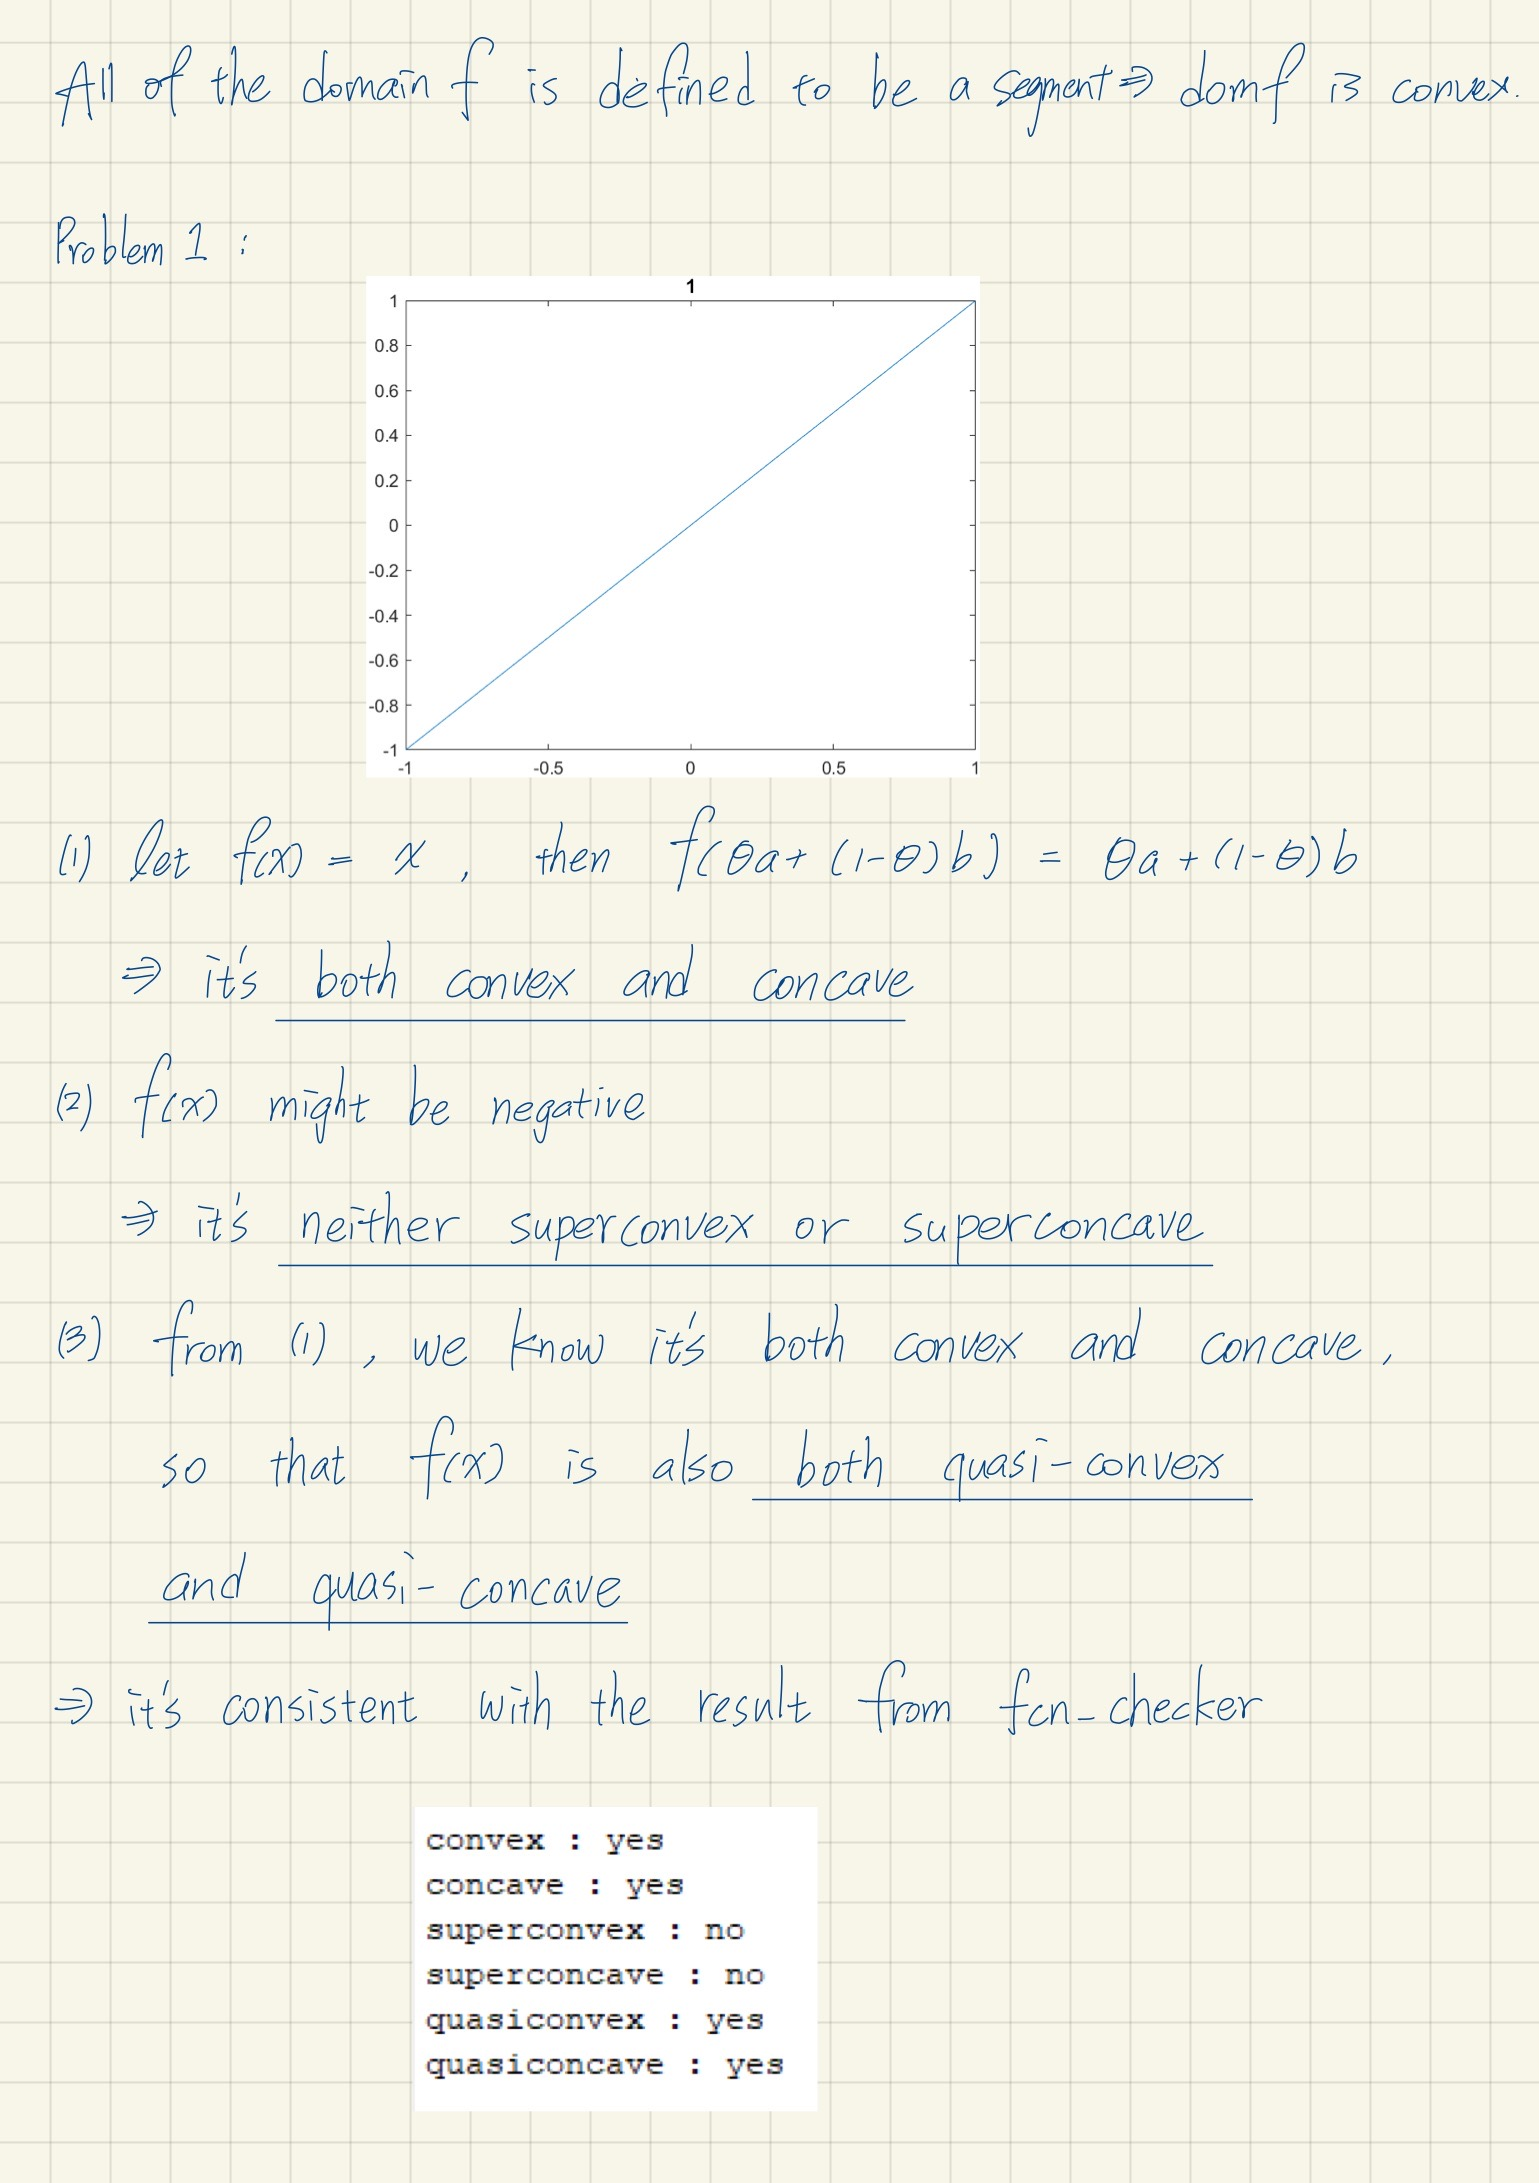
\includegraphics[width=1\textwidth]{proofs/prob1.jpg}
    \end{figure}

    \begin{figure}
        \centering
        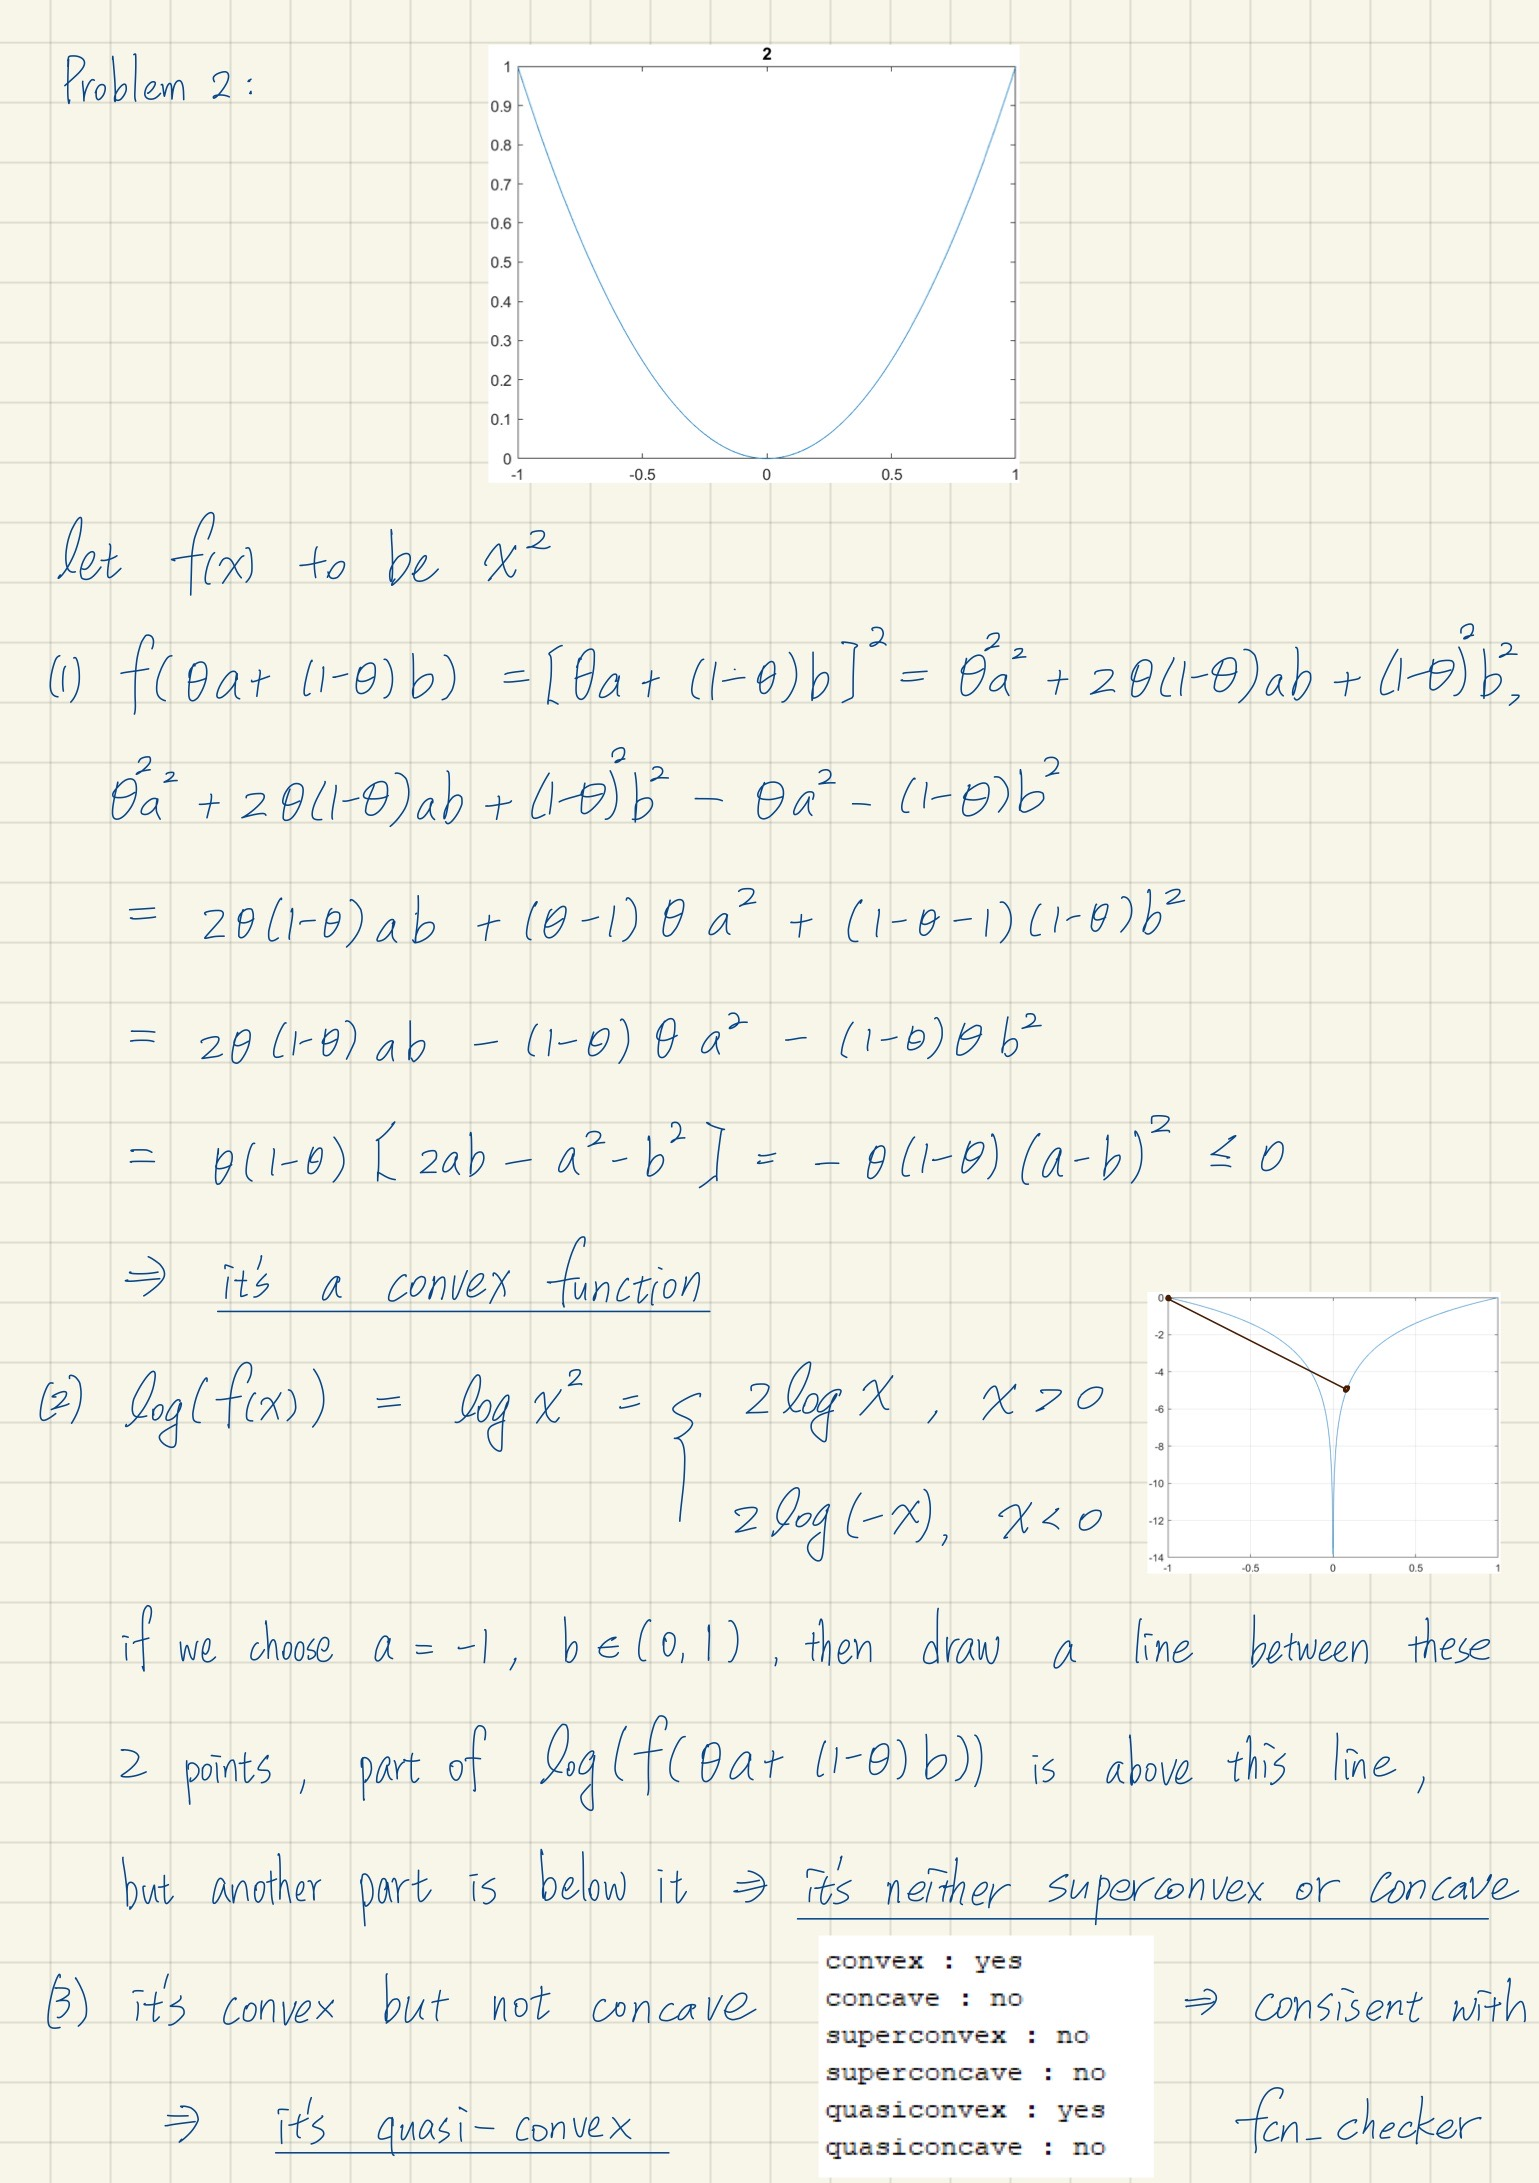
\includegraphics[width=1\textwidth]{proofs/prob2.jpg}
    \end{figure}

    \begin{figure}
        \centering
        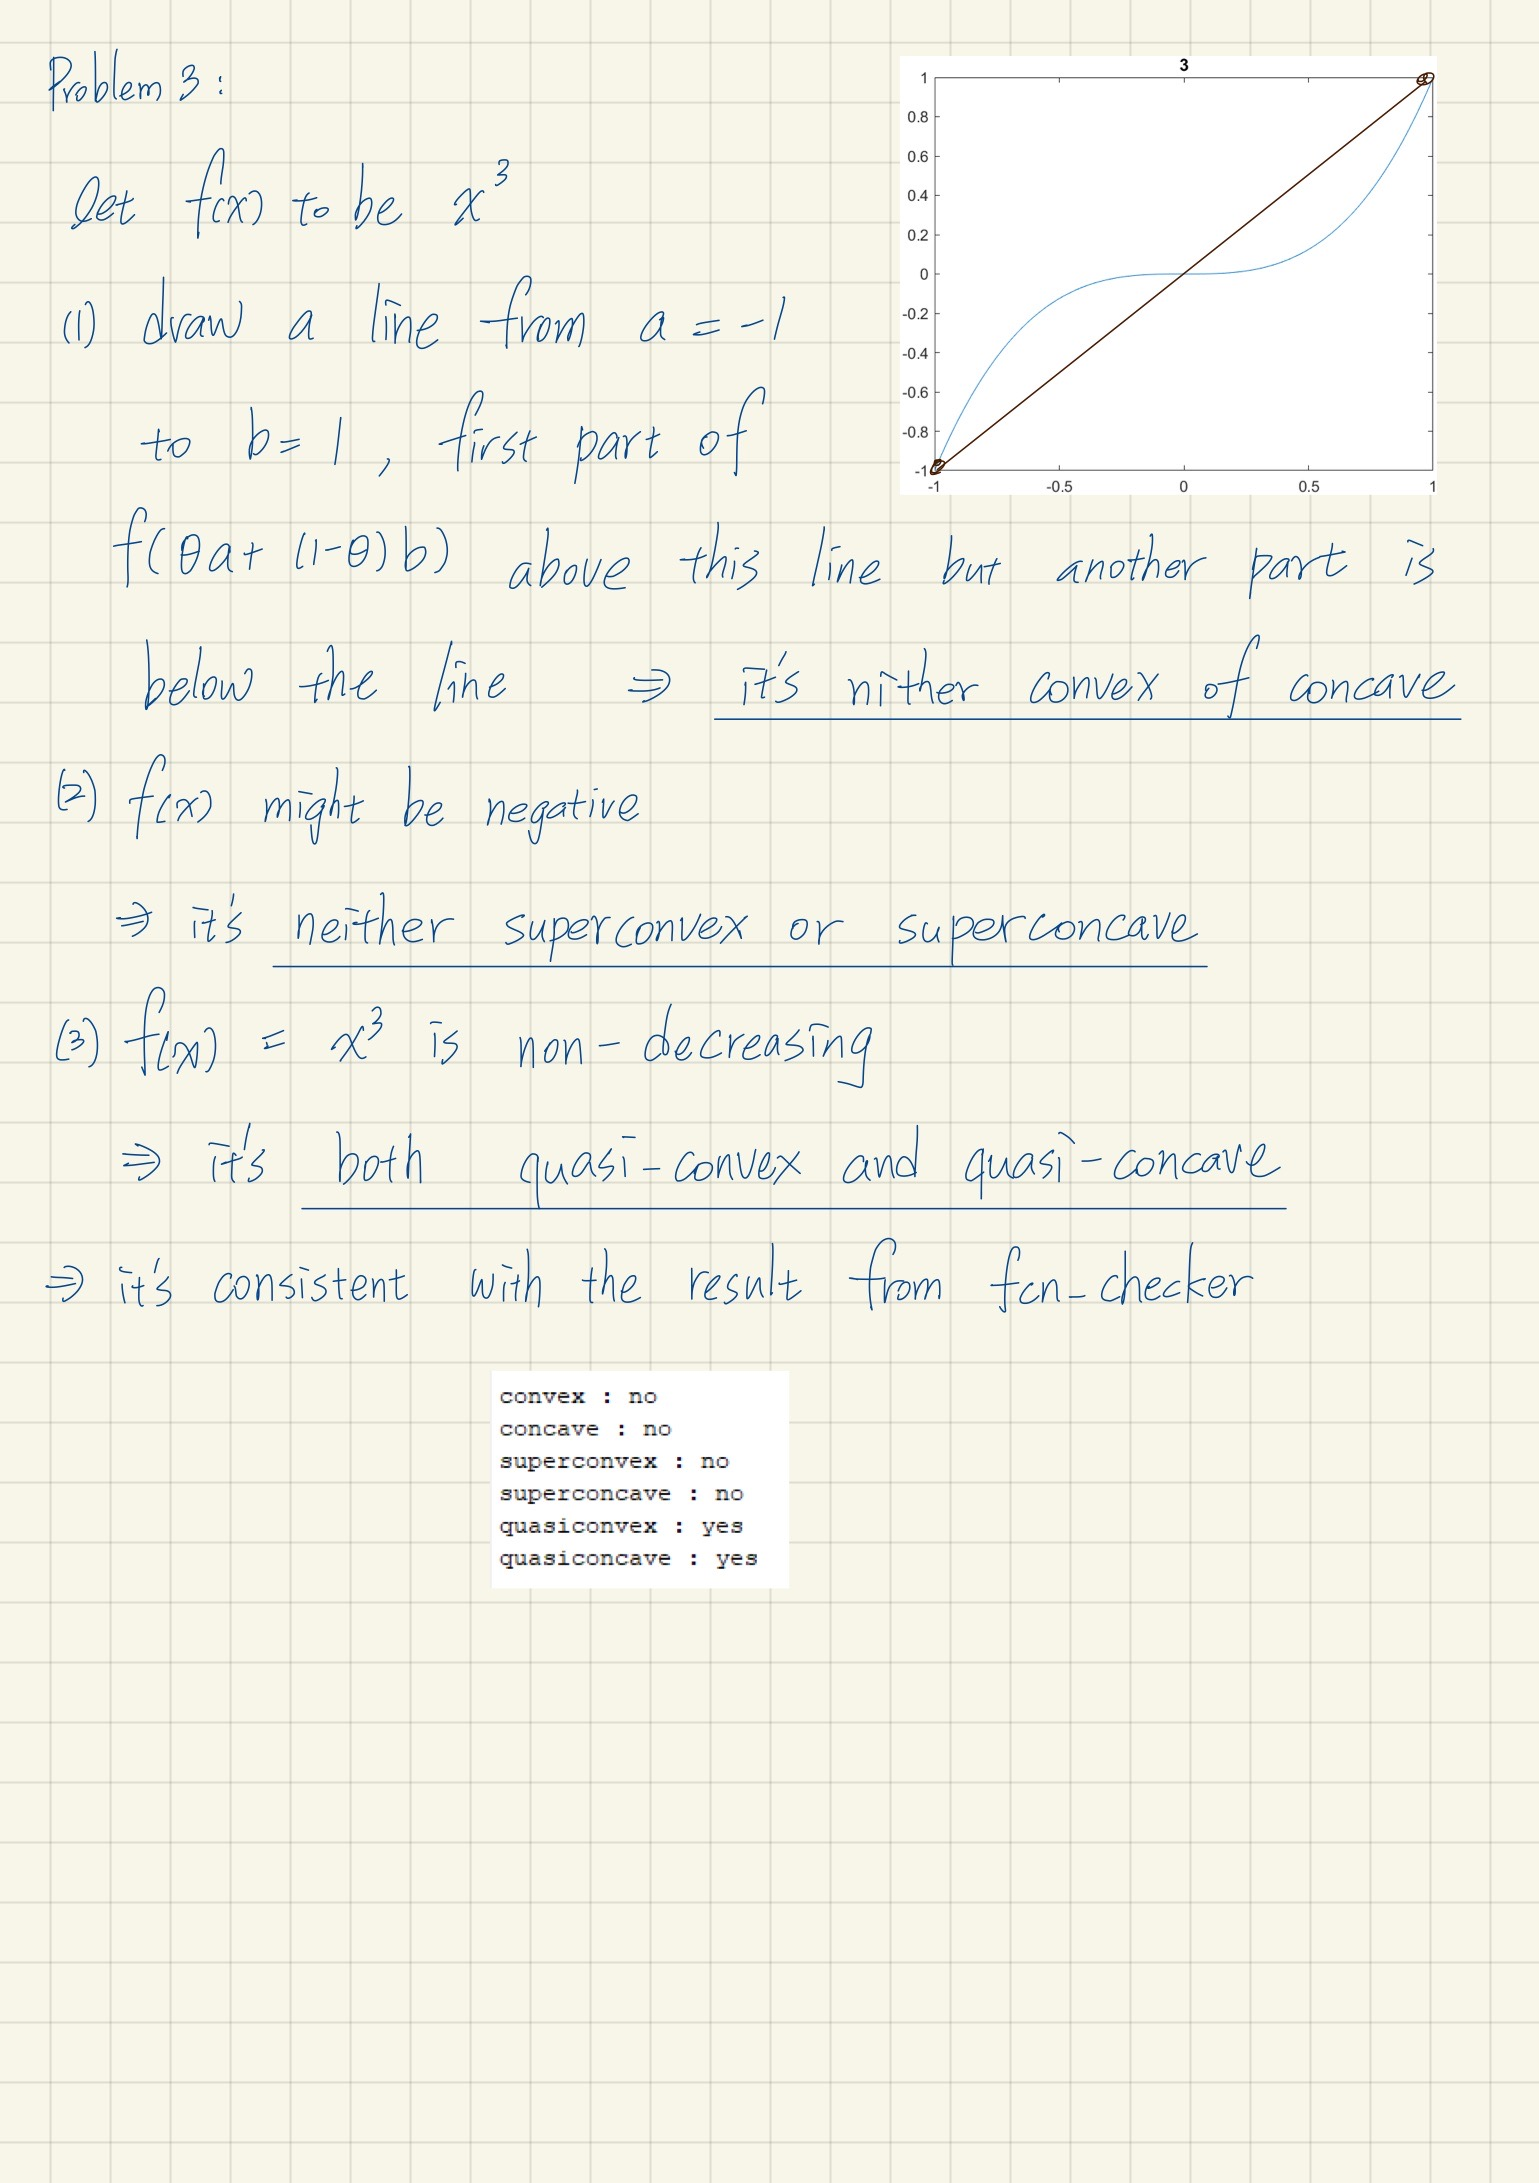
\includegraphics[width=1\textwidth]{proofs/prob3.jpg}
    \end{figure}

    \begin{figure}
        \centering
        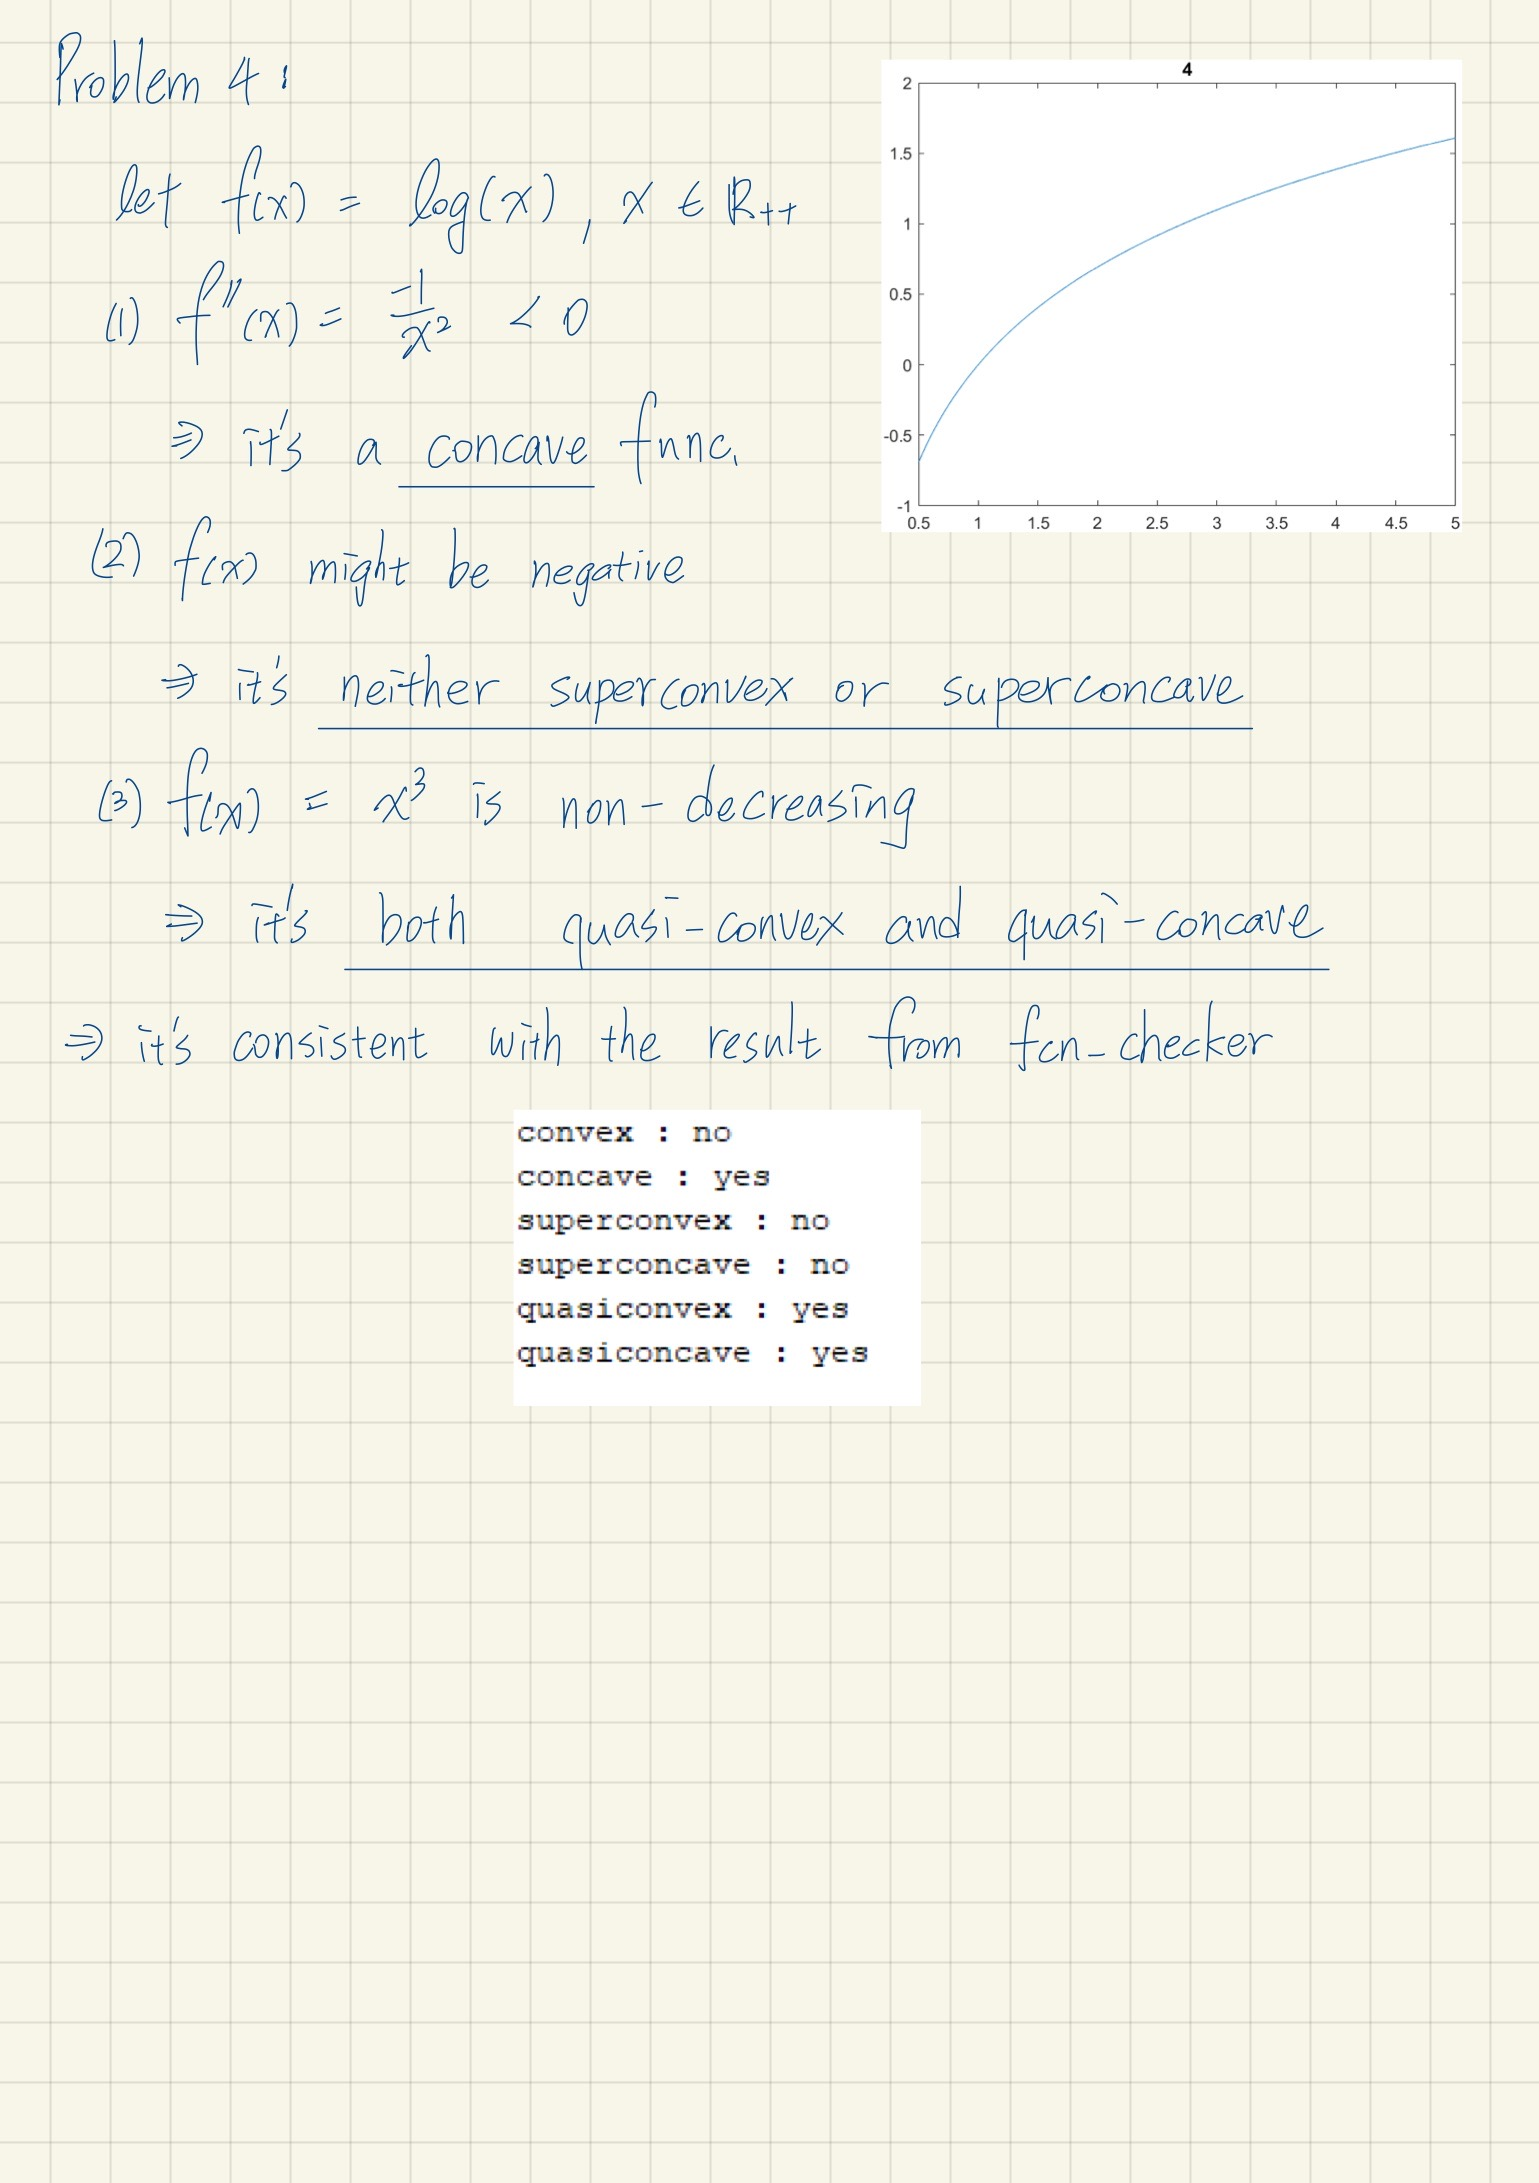
\includegraphics[width=1\textwidth]{proofs/prob4.jpg}
    \end{figure}

    \begin{figure}
        \centering
        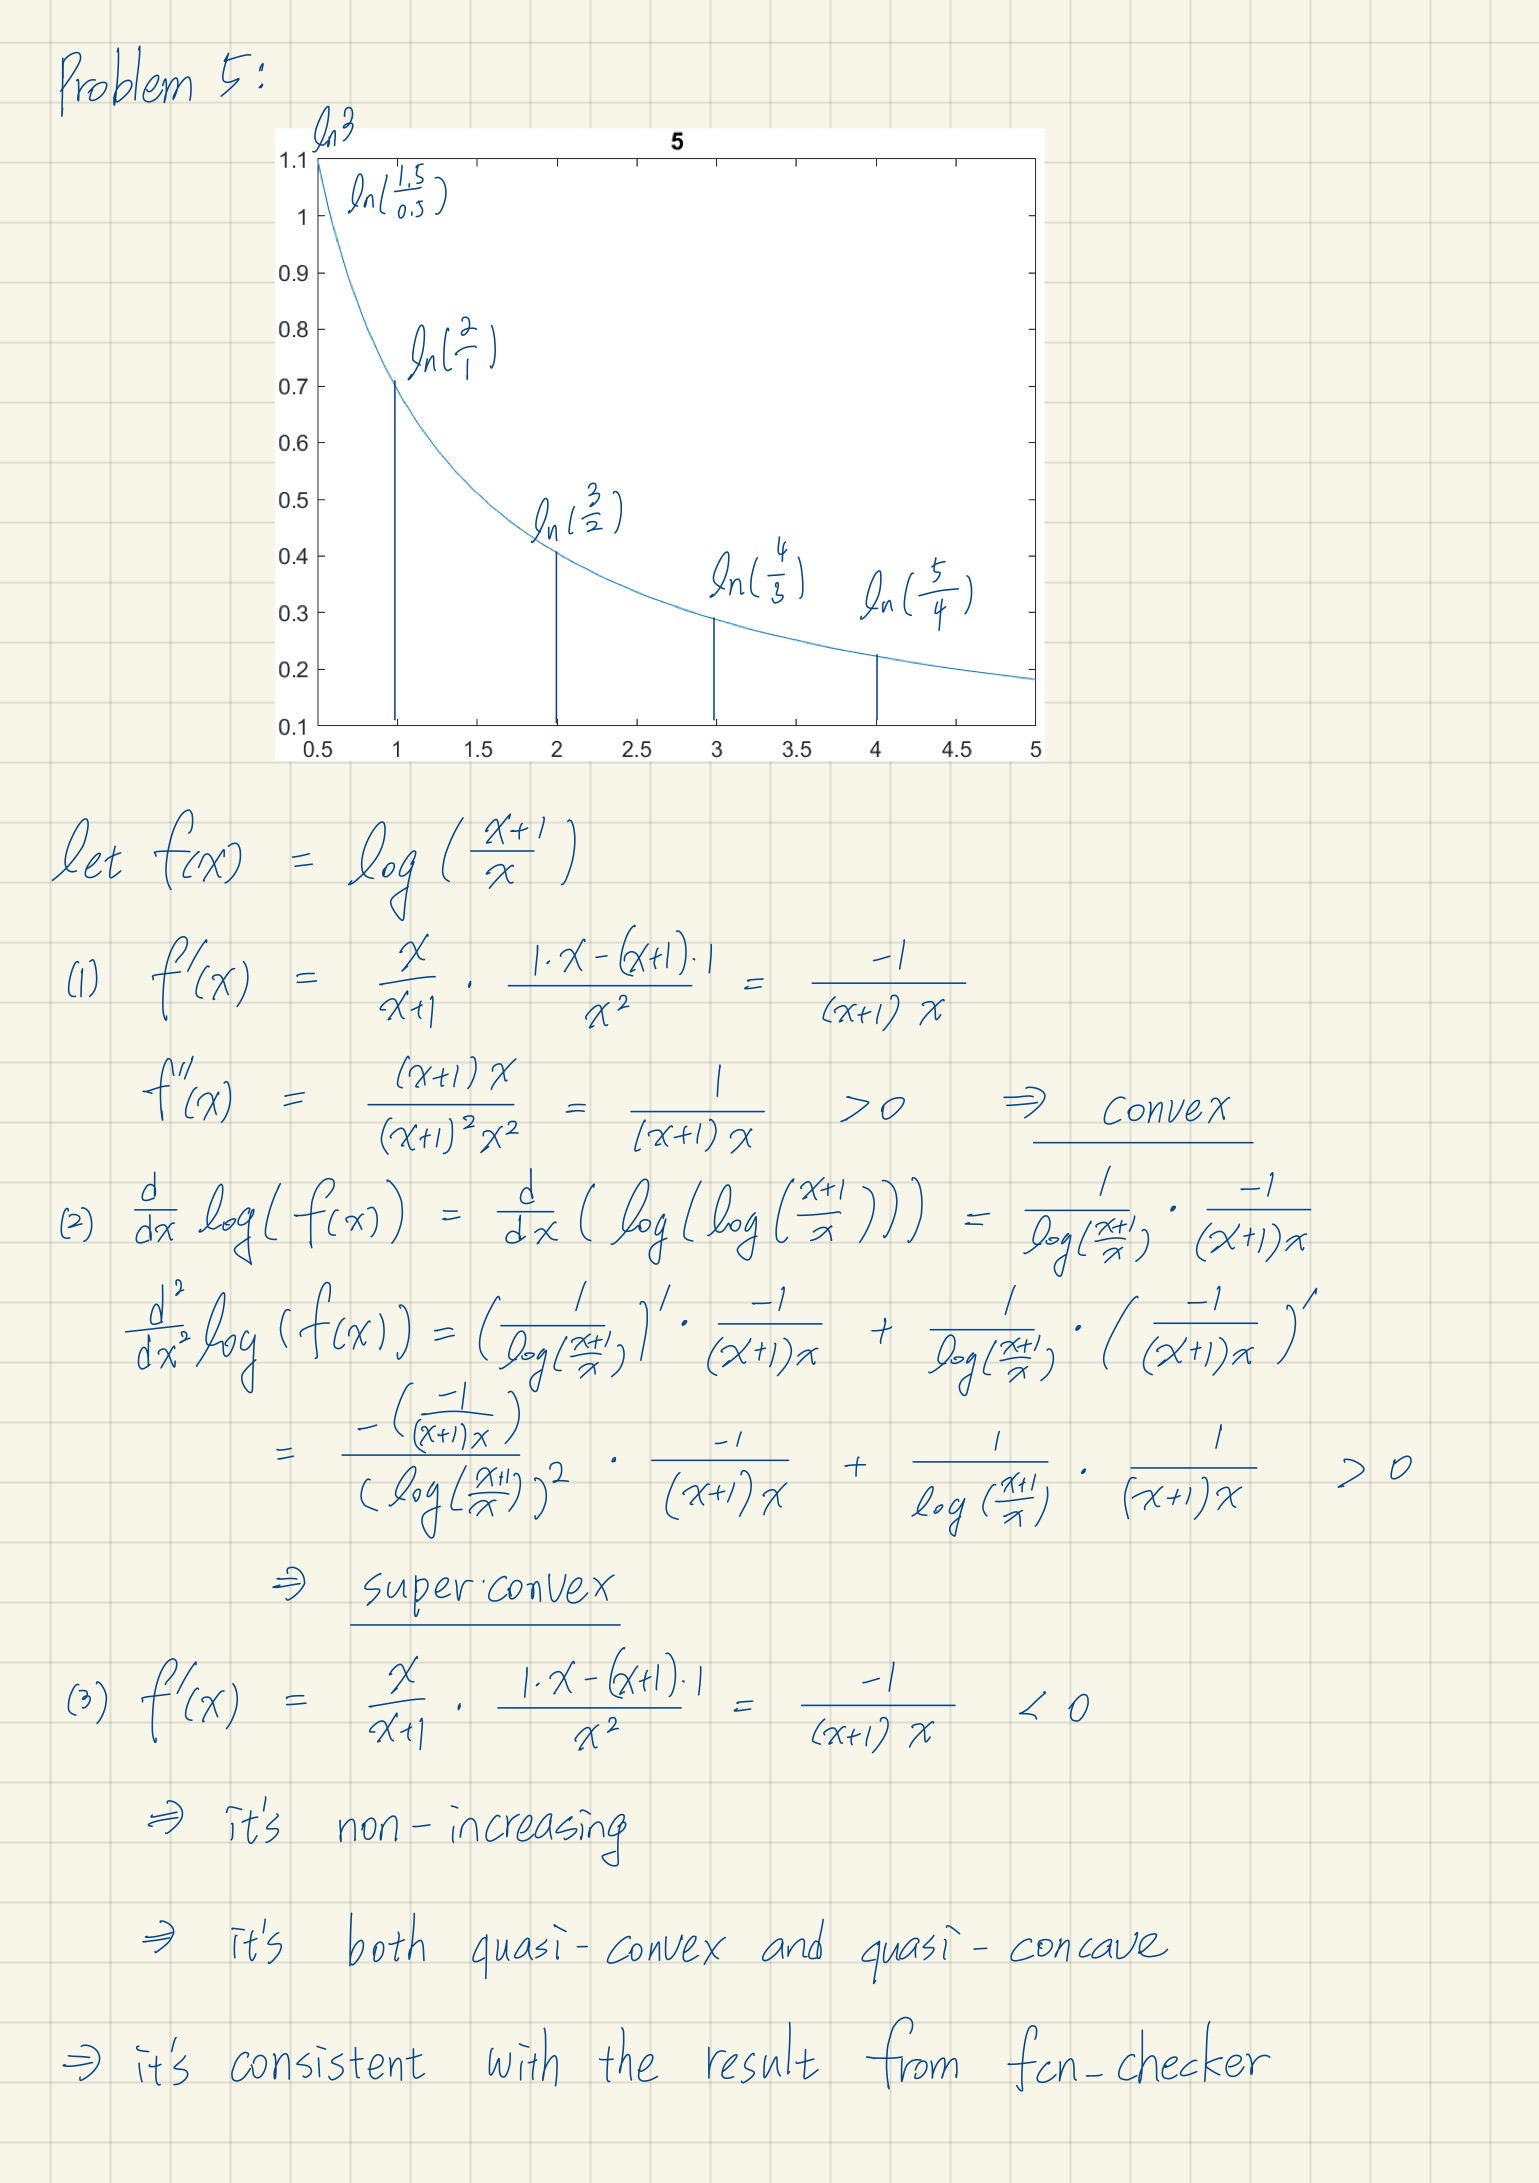
\includegraphics[width=1\textwidth]{proofs/prob5.jpg}
    \end{figure}


\end{document}




